%%%%%%%%%%%%%%%%%%%%%%%%%%%%%%%%%%%%%%%%%%%%%%%%%%%%%%%%%%%%%%%%%%%%%%%%%%%%%%%%%%%%%%%%%%%%%%%%%%%%%%%%%%%%%%%%%%%%%%%%%%%%%%%%%%%%%%%%%%%%%%%%%%%%%%
% 20141002 - Introduction to Operating Systems VO
%%%%%%%%%%%%%%%%%%%%%%%%%%%%%%%%%%%%%%%%%%%%%%%%%%%%%%%%%%%%%%%%%%%%%%%%%%%%%%%%%%%%%%%%%%%%%%%%%%%%%%%%%%%%%%%%%%%%%%%%%%%%%%%%%%%%%%%%%%%%%%%%%%%%%%

\tikzstyle{block} = [rectangle, draw, fill=blue!20, 
    text width=10em, text centered, rounded corners, minimum height=3em]
\tikzstyle{info} = [rectangle, draw, 
    text width=10em, text centered, rounded corners, minimum height=3em]

%fancyhdr
\lhead{IOS VO} 
\rhead{2014-10-02}

%%%%%%%%%%%%%%%%%%%%%%%%%%%%%%%%%%%%%%%%%%%%%%%%%%%%%%%%%%%%%%%%%%%%%%%%%%%%%%%%%%%%%%%%%%%%%%%%%%%%%%%%%%%%%%%%%%%%%%%%%%%%%%%%%%%%%%%%%%%%%%%%%%%%%%

\section*{Architecture}

%%%%%%%%%%%%%%%%%%%%%%%%%%%%%%%%%%%%%%%%%%%%%%%%%%%%%%%%%%%%%%%%%%%%%%%%%%%%%%%%%%%%%%%%%%%%%%%%%%%%%%%%%%%%%%%%%%%%%%%%%%%%%%%%%%%%%%%%%%%%%%%%%%%%%%

\par{
	\begin{figure}[!htb]
		\centering
		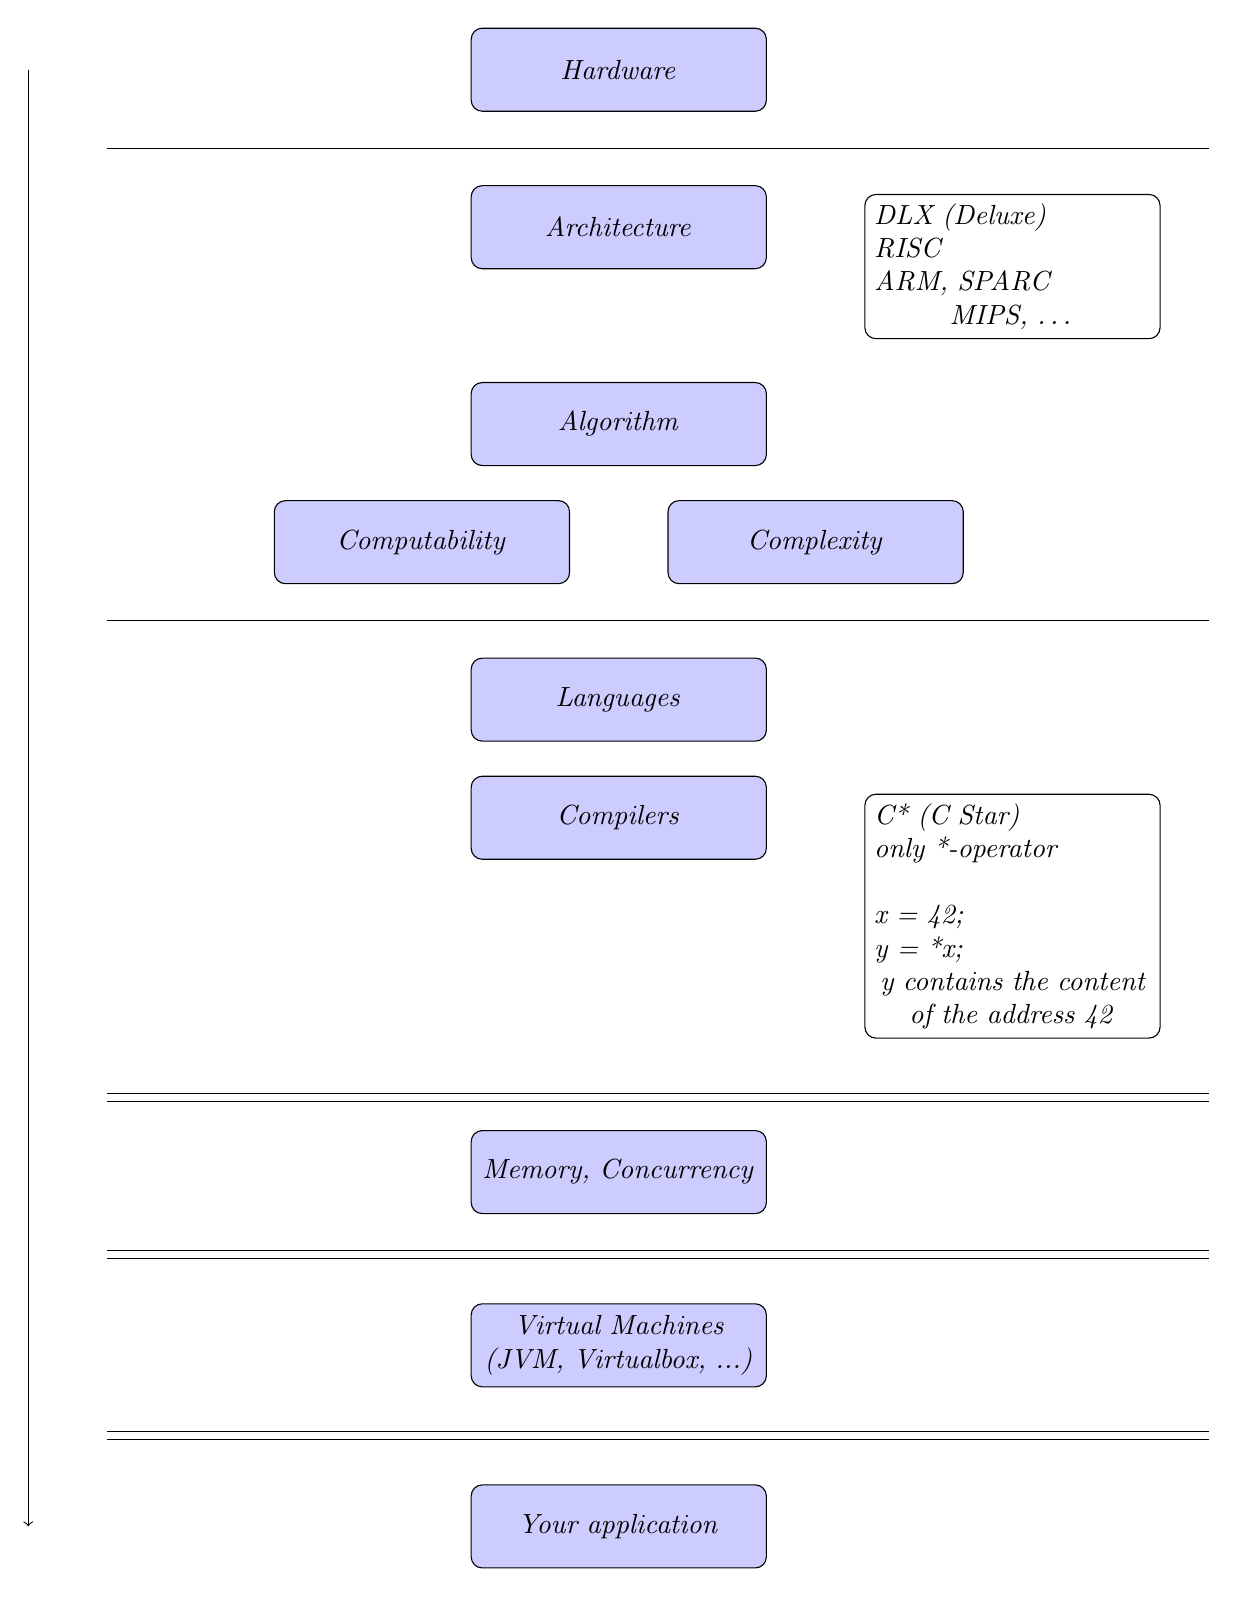
\begin{tikzpicture}[scale = 1.0]
			\draw[->] (0, 20) -- (0, 1.5);

			\node[block] (hardware) at (7.5, 20) {\textit{Hardware}};
            \draw (1, 19) -- (15, 19);
            
            \node[block] (architecture) at (7.5, 18) {\textit{Architecture}};
            \node[info] (archictectureinfo) at (12.5, 17.5) {\textit{DLX (Deluxe) \newline RISC \newline ARM, SPARC \newline MIPS, \ldots}};

            \node[block] (algorithm) at (7.5, 15.5) {\textit{Algorithm}};
            \node[block] (computability) at (5, 14) {\textit{Computability}};
            \node[block] (complexity) at (10, 14) {\textit{Complexity}};
            \draw (1, 13) -- (15, 13);

            \node[block] (languages) at (7.5, 12) {\textit{Languages}};
            \node[block] (compilers) at (7.5, 10.5) {\textit{Compilers}};
            \node[info] (compilersinfo) at (12.5, 9.25) {\textit{C* (C Star) \newline\noindent only *-operator \newline\newline x = 42; \newline y = *x; \newline y contains the content of the address 42}};
            
            \draw (1, 7) -- (15, 7);
            \draw (1, 6.90) -- (15, 6.90);
            
            \node[block] (memoryconcurrency) at (7.5, 6) {\textit{Memory, Concurrency}};

            \draw (1, 5) -- (15, 5);
            \draw (1, 4.90) -- (15, 4.90);

            \node[block] (virtualmachines) at (7.5, 3.8) {\textit{Virtual Machines (JVM, Virtualbox, ...)}};

            \draw (1, 2.7) -- (15, 2.7);
            \draw (1, 2.6) -- (15, 2.6);

            \node[block] (application) at (7.5, 1.5) {\textit{Your application}};
		\end{tikzpicture}
		\caption{Architecture hierarchy (top-down.}
		\label{fig:architecturehierarchy}
	\end{figure}
}

\section*{Von Neumann Architecture}

\par{
    \noindent
    Introduced in 1945. This is a stored program computer: data = program. The Fetch-Decode-Execute cycle (see Figure~\ref{fig:fetchdecodeexecute}) modifies the state of the machine.
}

\par{
	\begin{figure}[!htb]
		\centering
		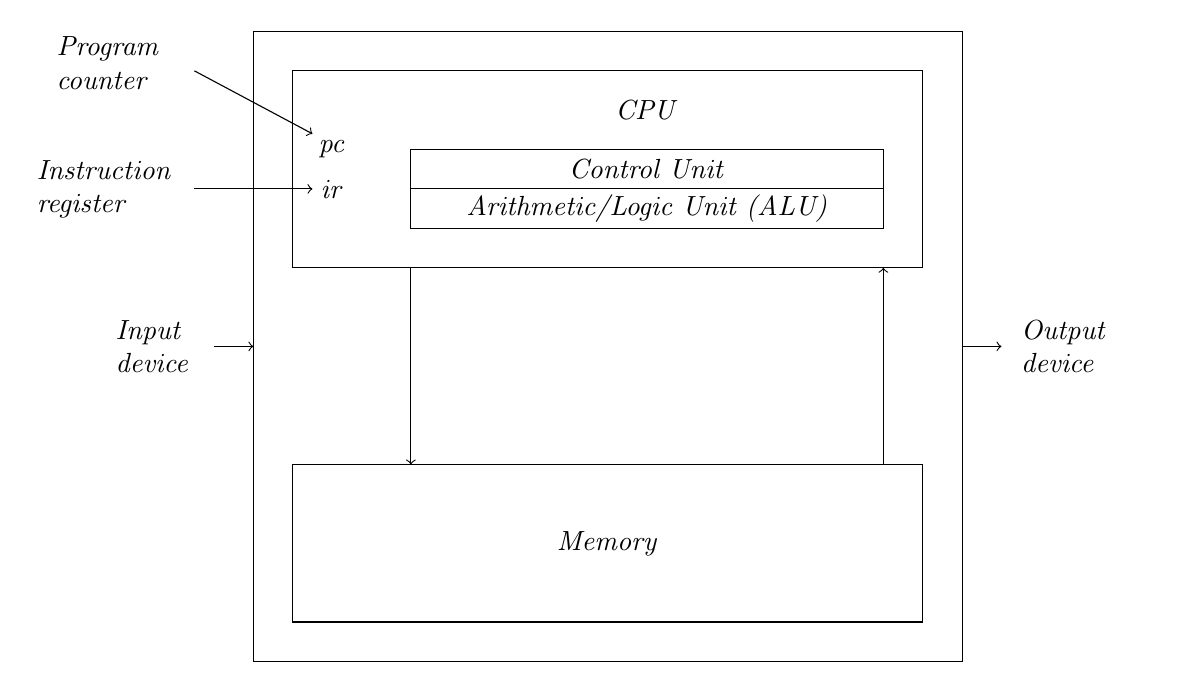
\begin{tikzpicture}
		    \draw (2, 0) rectangle (11, 8);

		    \draw (2.5, 5) rectangle (10.5, 7.5);
		    \node (cpu) at (7, 7) {\textit{CPU}};
		    \node (pc) at (3, 6.5) {\textit{pc}};
		    \node (ir) at (3, 6) {\textit{ir}};
		    \draw (4, 6) rectangle (10, 6.5) node[pos = 0.5]{\textit{Control Unit}};
		    \draw (4, 5.5) rectangle (10, 6) node[pos = 0.5]{\textit{Arithmetic/Logic Unit (ALU)}};

			\draw[->] (4, 5) -- (4, 2.5);
			\draw[<-] (10 , 5) -- (10, 2.5);

		    \draw (2.5, 0.5) rectangle (10.5, 2.5) node[pos = 0.5]{\textit{Memory}};

			\draw[->] (1.5, 4) -- (2, 4);
			\node (inputdevice) at (1, 4) [text width = 1.5cm]{\textit{Input device}};

			\draw[->] (11, 4) -- (11.5, 4);
			\node (outputdevice) at (12.5, 4) [text width = 1.5cm]{\textit{Output device}};

			\draw[->] (1.25, 7.5) -- (2.75, 6.7);
			\node (programcounter) at (0.25, 7.6) [text width = 1.5cm]{\textit{Program counter}};

			\draw[->] (1.25, 6) -- (2.75, 6);
			\node (instructionregister) at (0, 6) [text width = 1.5cm]{\textit{Instruction register}};
		\end{tikzpicture}
		\caption{Von Neumann Architecture.}
		\label{fig:vonneumann}
	\end{figure}
}

\par{
	\begin{figure}[!htb]
		\centering
		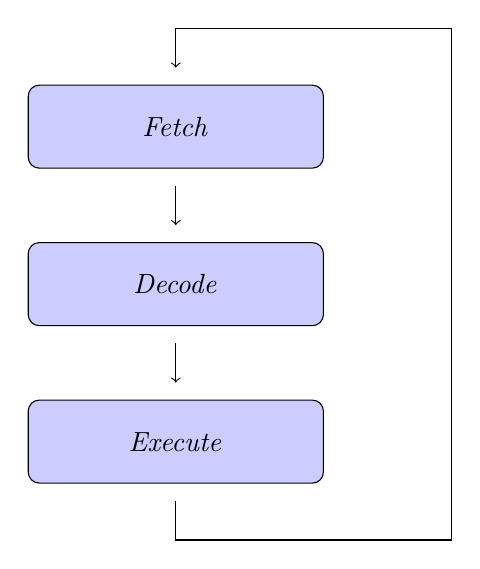
\begin{tikzpicture}
			\node[block] (fetch) at (0, 8) {\textit{Fetch}};
			\draw[->] (0, 7.25) -- (0, 6.75);
			\node[block] (decode) at (0, 6) {\textit{Decode}};
			\draw[->] (0, 5.25) -- (0, 4.75);
			\node[block] (execute) at (0, 4) {\textit{Execute}};
			\draw[->] (0, 3.25) -- (0, 2.75) -- (3.5, 2.75) -- (3.5, 9.25) -- (0, 9.25) -- (0, 8.75);
		\end{tikzpicture}
		\caption{Fetch-Decode-Execute cycle.}
		\label{fig:fetchdecodeexecute}
	\end{figure}
}
\clearpage

\subsection*{DLX Machine}

\par{
	\noindent
	\parskip0pt\begin{itemize}
		\item{Control unit: \newline
			Instruction register (ir) and program counter (pc).
		}
		\item{Arithmetic unit: \newline
			32x 32-bit registers; \texttt{reg[0]}, \texttt{reg[1]}, \ldots, \texttt{reg[31]}. \texttt{reg[0]} always contains the value \texttt{0} and \texttt{reg[31]} is the link register. Both are reserved by convention and must not be used for any other purpose.
		}
		\item{Memory: \newline
			n 32-bit words, byte-addressed (see Figure~\ref{fig:byteaddressedvisualization}), word-aligned; \newline \texttt{mem[0]}, \ldots, \texttt{mem[n - 1]}.
			\begin{figure}[!htb]
				\centering
				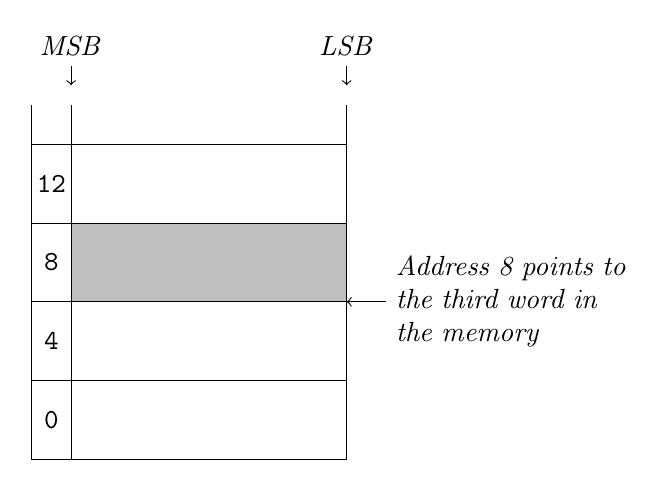
\begin{tikzpicture}
					\draw (0, 4.5) -- (0, 0) -- (4, 0) -- (4, 4.5);
					\draw (0.5, 4.5) -- (0.5, 0);
					\draw (0, 1) -- (4, 1);
					\draw (0, 2) -- (4, 2);
					\draw (0, 3) -- (4, 3);
					\draw (0, 4) -- (4, 4);

					\draw[<-] (0.5, 4.75) -- (0.5, 5) node[above] {\textit{MSB}};
					\draw[<-] (4, 4.75) -- (4, 5) node[above] {\textit{LSB}};
					
					\node at (0.25, 0.5) {\texttt{0}};
					\node at (0.25, 1.5) {\texttt{4}};
					\node at (0.25, 2.5) {\texttt{8}};
					\node at (0.25, 3.5) {\texttt{12}};

					\draw[fill = gray!50] (0.5, 2) rectangle (4, 3);

					\draw[<-] (4, 2) -- (4.5, 2) node[right, text width = 3cm] {\textit{Address 8 points to the third word in the memory}};
				\end{tikzpicture}
				\caption{Visualization of a byte-addressed memory of 32-bit words.}
				\label{fig:byteaddressedvisualization}
			\end{figure}
		}
	\end{itemize}
}

\clearpage

\subsection*{Syntax Formats}

\par{
	\noindent
	General syntax of an instruction: \texttt{op a, b, c}.
}

\subsubsection*{F1}

\par{
	\noindent
	The length of \texttt{a} and \texttt{b} allow to address all 32 registers. The two's complement is used here because the implementation of arithmetics is easier (in contrast to the one's complement).
	\begin{figure}[!htb]
		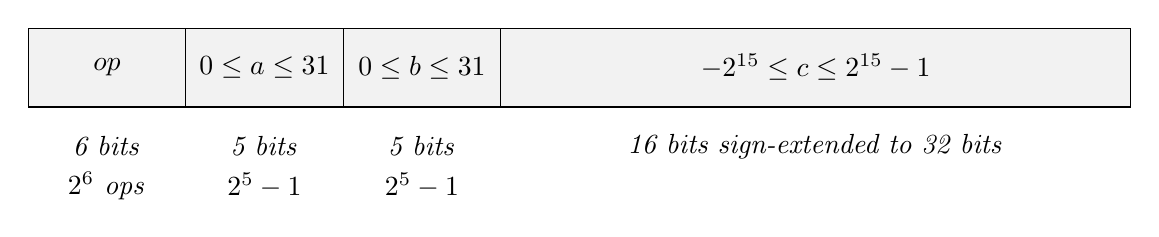
\begin{tikzpicture}
			\draw[fill = gray!10] (0, 1) rectangle (14, 2);
			
			\draw (2, 1) -- (2, 2);
			\node at (1, 1.5) {\texttt{$op$}};
			\node at (1, 0.5) {\textit{6 bits}};
			\node at (1, 0) {\textit{$2^6$ ops}};

			\draw (4, 1) -- (4, 2);
			\node at (3, 1.5) {\texttt{$0 \le a \le 31$}};
			\node at (3, 0.5) {\textit{5 bits}};
			\node at (3, 0) {\textit{$2^5 - 1$}};

			\draw (6, 1) -- (6, 2);
			\node at (5, 1.5) {\texttt{$0 \le b \le 31$}};
			\node at (5, 0.5) {\textit{5 bits}};
			\node at (5, 0) {\textit{$2^5 - 1$}};

			\node at (10, 1.5) {\texttt{$-2^{15} \le c \le 2^{15} - 1$}};
			\node at (10, 0.5) {\textit{16 bits sign-extended to 32 bits}};
		\end{tikzpicture}
	\end{figure}
}

\subsubsection*{F2}

\par{
	\noindent
	E.g. \texttt{R1 = R2 + R3}
	\begin{figure}[!htb]
		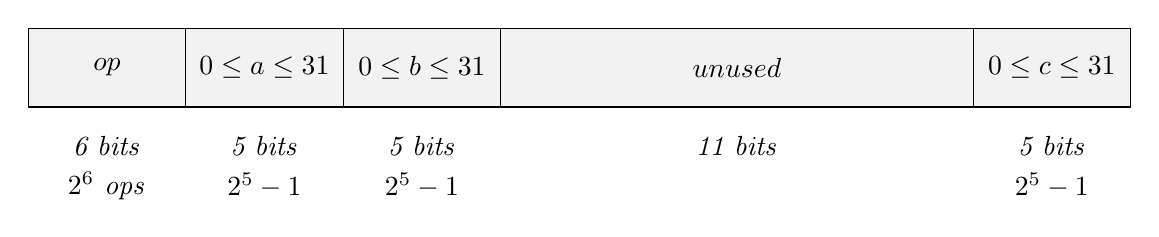
\begin{tikzpicture}
			\draw[fill = gray!10] (0, 1) rectangle (14, 2);
			
			\draw (2, 1) -- (2, 2);
			\node at (1, 1.5) {\texttt{$op$}};
			\node at (1, 0.5) {\textit{6 bits}};
			\node at (1, 0) {\textit{$2^6$ ops}};

			\draw (4, 1) -- (4, 2);
			\node at (3, 1.5) {\texttt{$0 \le a \le 31$}};
			\node at (3, 0.5) {\textit{5 bits}};
			\node at (3, 0) {\textit{$2^5 - 1$}};

			\draw (6, 1) -- (6, 2);
			\node at (5, 1.5) {\texttt{$0 \le b \le 31$}};
			\node at (5, 0.5) {\textit{5 bits}};
			\node at (5, 0) {\textit{$2^5 - 1$}};

			\draw (12, 1) -- (12, 2);
			\node at (9, 1.5) {\texttt{$unused$}};
			\node at (9, 0.5) {\textit{11 bits}};

			\node at (13, 1.5) {\texttt{$0 \le c \le 31$}};
			\node at (13, 0.5) {\textit{5 bits}};
			\node at (13, 0) {\textit{$2^5 - 1$}};
		\end{tikzpicture}
	\end{figure}
}

\subsubsection*{F3}

\par{
	\noindent
	Absolute addressing in memory.
	\begin{figure}[!htb]
		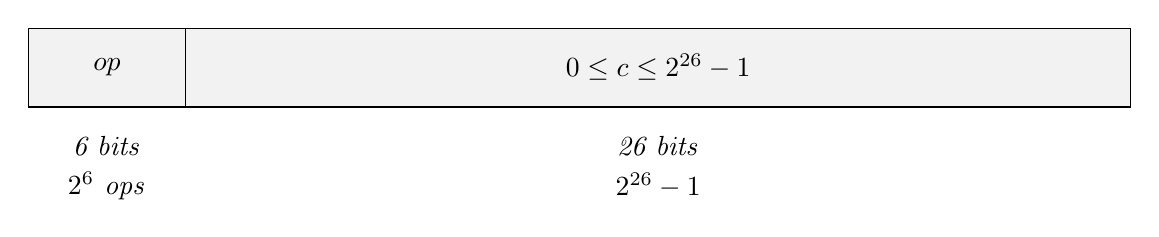
\begin{tikzpicture}
			\draw[fill = gray!10] (0, 1) rectangle (14, 2);
			
			\draw (2, 1) -- (2, 2);
			\node at (1, 1.5) {\texttt{$op$}};
			\node at (1, 0.5) {\textit{6 bits}};
			\node at (1, 0) {\textit{$2^6$ ops}};

			\node at (8, 1.5) {\texttt{$0 \le c \le 2^{26} - 1$}};
			\node at (8, 0.5) {\textit{26 bits}};
			\node at (8, 0) {\textit{$2^{26} - 1$}};
		\end{tikzpicture}
	\end{figure}
}

\par{
	\noindent
	\underline{Von Neumann Bottleneck:}	Memory read/write operations limit the performance.	
}

\clearpage

\subsection*{Register Instructions}

\subsubsection*{F1}

\par{
	\noindent
	\texttt{ADDI a, b, c}: Add immediate, \texttt{c} is data (a constant) \newline
	\texttt{reg[a] := reg[b] + c; pc := pc + 4;}
}

\par{
	\noindent
	\texttt{SUBI a, b, c}: Subtract immediate \newline
	\texttt{reg[a] := reg[b] - c; pc := pc + 4;}
}
